\chapter{Mouvements circulaires uniformes}

\textit{Le mouvement circulaire uniforme est un mouvement fondamental en physique, des particules élémentaires aux satellites en orbite. Ce chapitre explore les caractéristiques de ce mouvement, l'accélération centripète qui le régit, et ses applications majeures : le mouvement d'une particule chargée dans un champ magnétique uniforme (cyclotron, spectrographe de masse) et le mouvement des satellites et planètes sous l'effet de la gravitation (lois de Kepler, satellites géostationnaires, vitesses cosmiques).}

\section{Caractéristiques du mouvement circulaire uniforme}

\subsection{Définition et repérage}

\begin{definition}[Mouvement circulaire uniforme]
Un point matériel $M$ décrit un mouvement circulaire uniforme (MCU) si sa trajectoire est un cercle et si la valeur de sa vitesse $v$ est constante.
\end{definition}

Pour repérer $M$ sur un cercle de rayon $R$ et de centre $O$, on utilise l'abscisse curviligne $s(t)$ (longueur de l'arc parcouru) ou l'angle polaire $\theta(t)$ (en radians). La relation entre $s$ et $\theta$ est :
\[
s(t) = R\,\theta(t)
\]

\begin{propriete}[Vitesse angulaire]
La vitesse angulaire $\omega$ (en \si{\radian\per\second}) est définie par :
\[
\omega = \frac{\mathrm{d}\theta}{\mathrm{d}t} = \dot{\theta}
\]
Pour un MCU, $\omega$ est constante. La vitesse linéaire $v$ (en \si{\metre\per\second}) est liée à $\omega$ par :
\[
v = R\,\omega
\]
\end{propriete}

\begin{remarque}
La période $T$ (temps pour un tour complet) et la fréquence $f$ (nombre de tours par seconde) sont liées à $\omega$ par :
\[
\omega = \frac{2\pi}{T} = 2\pi f
\]
\end{remarque}

\subsection{Accélération centripète}

\begin{loi}[Accélération dans le MCU]
Dans un mouvement circulaire uniforme, l'accélération est centripète : elle est dirigée vers le centre $O$ du cercle et sa valeur est constante :
\[
\vect{a} = -\frac{v^2}{R}\,\vect{u}_r = -R\omega^2\,\vect{u}_r
\]
où $\vect{u}_r$ est le vecteur unitaire radial dirigé de $O$ vers $M$. La norme de l'accélération est :
\[
a = \frac{v^2}{R} = R\omega^2
\]
\end{loi}

\begin{experience}[Mise en évidence de l'accélération centripète]
Une bille attachée à un fil tourne dans un plan horizontal. Si le fil casse, la bille s'échappe tangentiellement, montrant que la force centripète (tension du fil) maintenait le mouvement circulaire.
\end{experience}

\begin{aretenir}
Dans un MCU, la vitesse est tangente à la trajectoire, l'accélération est radiale et centripète. Il n'y a pas d'accélération tangentielle.
\end{aretenir}

\section{Particule chargée dans un champ magnétique uniforme}

\subsection{Force de Lorentz}

\begin{loi}[Force de Lorentz]
Une particule de charge $q$ se déplaçant à la vitesse $\vect{v}$ dans un champ magnétique $\vect{B}$ subit la force de Lorentz :
\[
\vect{F}_L = q\,\vect{v} \wedge \vect{B}
\]
Cette force est toujours perpendiculaire à $\vect{v}$ et à $\vect{B}$.
\end{loi}

\begin{propriete}[Travail de la force de Lorentz]
La force de Lorentz ne travaille pas ($\vect{F}_L \perp \vect{v}$), donc l'énergie cinétique de la particule reste constante. Seule la direction de la vitesse change.
\end{propriete}

\subsection{Mouvement dans un champ $\vect{B}$ uniforme}

Considérons une particule de masse $m$ et de charge $q$ pénétrant avec une vitesse $\vect{v}_0$ perpendiculaire à $\vect{B}$ (champ uniforme, entrant dans la page).

\begin{illus}
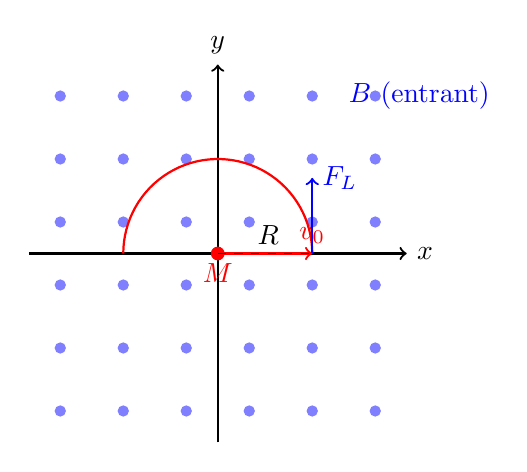
\begin{tikzpicture}[scale=0.8]
  \draw[thick,->] (-3,0) -- (3,0) node[right]{$x$};
  \draw[thick,->] (0,-3) -- (0,3) node[above]{$y$};
  \foreach \x in {-2.5,-1.5,...,2.5}
    \foreach \y in {-2.5,-1.5,...,2.5}
      \filldraw[blue!50] (\x,\y) circle (0.08);
  \node[blue] at (3.2,2.5){$\vect{B}$ (entrant)};
  \draw[thick,->,red] (0,0) -- (1.5,0) node[above]{$\vect{v}_0$};
  \draw[thick,red,domain=0:180,samples=50] plot ({1.5*cos(\x)},{1.5*sin(\x)});
  \filldraw[red] (0,0) circle (0.1) node[below]{$M$};
  \draw[thick,->,blue] (1.5,0) -- (1.5,1.2) node[right]{$\vect{F}_L$};
  \draw[dashed] (0,0) -- (1.5,0);
  \node at (0.8,0.3){$R$};
\end{tikzpicture}
\fig{Figure 4.1 — Trajectoire circulaire d'une particule chargée dans un champ magnétique uniforme $\vect{B}$ perpendiculaire à $\vect{v}_0$.}
\end{illus}

\begin{propriete}[Rayon de courbure et période cyclotron]
Sous l'effet de la force de Lorentz, la particule décrit un mouvement circulaire uniforme dans le plan perpendiculaire à $\vect{B}$. Le rayon $R$ de la trajectoire et la période $T$ (période cyclotron) sont :
\[
R = \frac{mv}{|q|B} \qquad ; \qquad T = \frac{2\pi m}{|q|B}
\]
La période $T$ est indépendante de la vitesse $v$ (propriété fondamentale pour le cyclotron).
\end{propriete}

\begin{exemple}
Un proton ($m=\SI{1.67e-27}{\kilogram}$, $q=\SI{1.6e-19}{\coulomb}$) pénètre dans un champ $\vect{B}=\SI{0.5}{\tesla}$ avec $v=\SI{2e6}{\metre\per\second}$. Calculer $R$ et $T$.
\[
R = \frac{1.67\times10^{-27}\times2\times10^{6}}{1.6\times10^{-19}\times0.5} = \SI{0.042}{\metre} = \SI{4.2}{\centi\metre}
\]
\[
T = \frac{2\pi\times1.67\times10^{-27}}{1.6\times10^{-19}\times0.5} = \SI{1.31e-7}{\second}
\]
\end{exemple}

\subsection{Applications : spectrographe de masse et cyclotron}

\begin{experience}[Spectrographe de masse]
Un spectrographe de masse sépare des ions de masses différentes. Les ions sont accélérés par une tension $U$, puis déviés par un champ $\vect{B}$. Le rayon de courbure $R$ dépend de $m$ :
\[
R = \frac{1}{B}\sqrt{\frac{2mU}{q}}
\]
En mesurant $R$, on détermine $m$.
\end{experience}

\begin{experience}[Cyclotron]
Le cyclotron accélère des particules chargées en utilisant un champ magnétique constant et un champ électrique alternatif. La fréquence du champ électrique doit être égale à la fréquence cyclotron $f = \frac{|q|B}{2\pi m}$.
\end{experience}

\section{Satellites et planètes — Gravitation}

\subsection{Loi de la gravitation universelle}

\begin{loi}[Loi de Newton]
Deux corps ponctuels $A$ et $B$ de masses $m_A$ et $m_B$ séparés par une distance $r$ exercent l'un sur l'autre une force attractive :
\[
\vect{F}_{A\to B} = -G\,\frac{m_A m_B}{r^2}\,\vect{u}_{AB}
\]
où $G=\SI{6.67e-11}{\newton\metre\squared\per\kilogram\squared}$ est la constante de gravitation universelle.
\end{loi}

\subsection{Mouvement des satellites et planètes}

\begin{loi}[Lois de Kepler]
\begin{enumerate}
\item \textbf{Loi des orbites} : Les planètes décrivent des orbites elliptiques dont le Soleil occupe l'un des foyers.
\item \textbf{Loi des aires} : Le rayon vecteur Soleil-planète balaie des aires égales pendant des durées égales.
\item \textbf{Loi des périodes} : Le carré de la période de révolution $T$ est proportionnel au cube du demi-grand axe $a$ de l'orbite :
\[
\frac{T^2}{a^3} = \text{constante}
\]
Pour une orbite circulaire de rayon $r$ autour d'un astre de masse $M$ :
\[
T^2 = \frac{4\pi^2}{GM}\,r^3
\]
\end{enumerate}
\end{loi}

\begin{propriete}[Satellite en orbite circulaire]
Un satellite de masse $m$ en orbite circulaire de rayon $r$ autour d'un astre de masse $M$ ($M \gg m$) a une vitesse $v$ et une période $T$ :
\[
v = \sqrt{\frac{GM}{r}} \qquad ; \qquad T = 2\pi\sqrt{\frac{r^3}{GM}}
\]
\end{propriete}

\begin{illus}
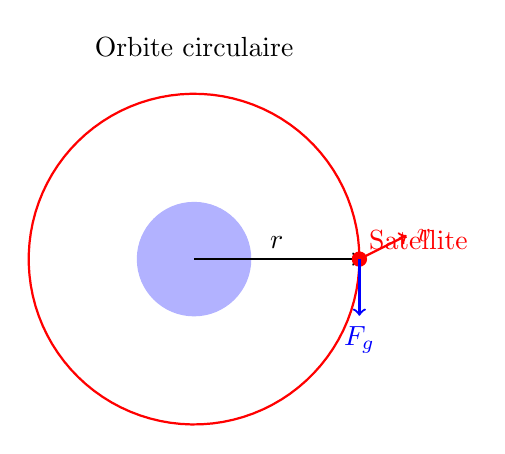
\begin{tikzpicture}[scale=0.6]
  \filldraw[blue!30] (0,0) circle (1.2) node{$\oplus$};
  \draw[thick,->] (0,0) -- (3.5,0) node[midway,above]{$r$};
  \draw[thick,red,domain=0:360,samples=100] plot ({3.5*cos(\x)},{3.5*sin(\x)});
  \filldraw[red] (3.5,0) circle (0.15) node[above right]{Satellite};
  \draw[thick,->,red] (3.5,0) -- (4.5,0.5) node[right]{$\vect{v}$};
  \draw[thick,->,blue] (3.5,0) -- (3.5,-1.2) node[below]{$\vect{F}_g$};
  \node at (0,4.5){Orbite circulaire};
\end{tikzpicture}
\fig{Figure 4.2 — Satellite en orbite circulaire autour de la Terre. La force gravitationnelle $\vect{F}_g$ fournit l'accélération centripète.}
\end{illus}

\subsection{Satellite géostationnaire}

\begin{definition}[Satellite géostationnaire]
Un satellite géostationnaire est un satellite qui reste fixe par rapport à un point de la surface terrestre. Il doit :
\begin{itemize}
\item Être en orbite circulaire dans le plan équatorial.
\item Tourner dans le même sens que la Terre (ouest-est).
\item Avoir une période $T = \SI{24}{\hour} = \SI{86400}{\second}$.
\end{itemize}
\end{definition}

\begin{exemple}
Calculer l'altitude $h$ d'un satellite géostationnaire ($R_T = \SI{6370}{\kilo\metre}$, $M_T = \SI{5.97e24}{\kilogram}$).
\[
T^2 = \frac{4\pi^2}{GM_T}\,(R_T+h)^3 \Rightarrow (R_T+h)^3 = \frac{GM_T T^2}{4\pi^2}
\]
\[
R_T+h = \sqrt[3]{\frac{6.67\times10^{-11}\times5.97\times10^{24}\times(86400)^2}{4\pi^2}} \approx \SI{4.22e7}{\metre}
\]
\[
h = 4.22\times10^7 - 6.37\times10^6 = \SI{3.58e7}{\metre} \approx \SI{35800}{\kilo\metre}
\]
\end{exemple}

\subsection{Vitesses cosmiques}

\begin{propriete}[Vitesses cosmiques]
\begin{itemize}
\item \textbf{Vitesse de libération (2\up{e} vitesse cosmique)} : vitesse minimale pour quitter l'attraction terrestre depuis la surface :
\[
v_2 = \sqrt{\frac{2GM_T}{R_T}} \approx \SI{11.2}{\kilo\metre\per\second}
\]
\item \textbf{Vitesse de satellisation (1\up{re} vitesse cosmique)} : vitesse pour une orbite circulaire rasante ($r=R_T$) :
\[
v_1 = \sqrt{\frac{GM_T}{R_T}} \approx \SI{7.9}{\kilo\metre\per\second}
\]
\end{itemize}
\end{propriete}

\begin{aretenir}
La force gravitationnelle joue le rôle de force centripète pour les satellites en orbite. La vitesse orbitale diminue quand $r$ augmente.
\end{aretenir}

\section{L'essentiel à retenir}

\begin{synthese}
\begin{itemize}
\item \textbf{MCU} : $v = R\omega$, $a = v^2/R = R\omega^2$ (centripète).
\item \textbf{Particule chargée dans $\vect{B}$} : $R = mv/(|q|B)$, $T = 2\pi m/(|q|B)$ (indépendant de $v$).
\item \textbf{Gravitation} : $F = G m_1 m_2 / r^2$.
\item \textbf{Satellite circulaire} : $v = \sqrt{GM/r}$, $T = 2\pi\sqrt{r^3/(GM)}$.
\item \textbf{Géostationnaire} : $T = \SI{24}{\hour}$, orbite équatoriale, $h \approx \SI{35800}{\kilo\metre}$.
\item \textbf{Vitesses cosmiques} : $v_1 = \sqrt{GM/R} \approx \SI{7.9}{\kilo\metre\per\second}$, $v_2 = \sqrt{2GM/R} \approx \SI{11.2}{\kilo\metre\per\second}$.
\end{itemize}
\end{synthese}

\section{Méthodes \& savoir-faire}

\methode{Déterminer l'accélération dans un MCU}
Utiliser $a = v^2/R = R\omega^2$. Vérifier que la direction est centripète.

\begin{exemple}
Un disque de rayon $R=\SI{0.2}{\metre}$ tourne à $f=\SI{10}{\hertz}$. Calculer $a$ en un point de la périphérie.
\[
\omega = 2\pi f = 20\pi\ \si{\radian\per\second},\quad a = R\omega^2 = 0.2\times(20\pi)^2 \approx \SI{789.6}{\metre\per\second\squared}
\]
\end{exemple}

\methode{Calculer le rayon de courbure d'une particule dans $\vect{B}$}
Appliquer $R = mv/(|q|B)$. Attention aux unités (SI).

\begin{exemple}
Un électron ($m=\SI{9.11e-31}{\kilogram}$, $q=\SI{-1.6e-19}{\coulomb}$) a $v=\SI{3e6}{\metre\per\second}$ dans $B=\SI{0.02}{\tesla}$. $R = \frac{9.11\times10^{-31}\times3\times10^{6}}{1.6\times10^{-19}\times0.02} \approx \SI{8.54e-4}{\metre} = \SI{0.854}{\milli\metre}$.
\end{exemple}

\methode{Appliquer la 3\up{e} loi de Kepler}
Pour un satellite, $T^2/r^3 = 4\pi^2/(GM)$. Utiliser cette constante pour relier deux orbites.

\begin{exemple}
Deux satellites $S_1$ ($r_1=\SI{7000}{\kilo\metre}$, $T_1=\SI{1.5}{\hour}$) et $S_2$ ($r_2=\SI{14000}{\kilo\metre}$). Calculer $T_2$.
\[
\frac{T_2^2}{r_2^3} = \frac{T_1^2}{r_1^3} \Rightarrow T_2 = T_1\sqrt{\frac{r_2^3}{r_1^3}} = 1.5\times\sqrt{8} \approx \SI{4.24}{\hour}
\]
\end{exemple}

\methode{Déterminer l'altitude d'un satellite géostationnaire}
Utiliser $T = \SI{86400}{\second}$, $r = R_T + h$, et $T^2 = 4\pi^2 r^3/(GM_T)$.

\methode{Calculer une vitesse cosmique}
$v_1 = \sqrt{GM/R}$, $v_2 = \sqrt{2GM/R}$. Utiliser $M_T$ et $R_T$.

\methode{Analyser le mouvement d'un satellite}
La force gravitationnelle fournit l'accélération centripète : $GMm/r^2 = mv^2/r$.

\section{Exercices d'application}

\rubrique{Mouvement circulaire uniforme}

\exo{}\diff{1} Un point $M$ parcourt un cercle de rayon $R=\SI{0.5}{\metre}$ à la vitesse constante $v=\SI{2}{\metre\per\second}$. Calculer $\omega$, $T$ et $f$.

\exo{}\diff{2} Un disque de rayon $R=\SI{0.3}{\metre}$ tourne à $\omega=\SI{10}{\radian\per\second}$. Calculer la vitesse linéaire $v$ et l'accélération $a$ d'un point de la périphérie.

\exo{}\diff{2} Un satellite artificiel tourne autour de la Terre sur une orbite circulaire de rayon $r=\SI{8000}{\kilo\metre}$. Sa période est $T=\SI{2}{\hour}$. Calculer sa vitesse $v$ et son accélération $a$.

\rubrique{Particule chargée dans un champ magnétique}

\exo{}\diff{1} Un proton ($m=\SI{1.67e-27}{\kilogram}$, $q=\SI{1.6e-19}{\coulomb}$) pénètre dans un champ $B=\SI{0.1}{\tesla}$ avec $v=\SI{1e5}{\metre\per\second}$ perpendiculaire à $\vect{B}$. Calculer $R$ et $T$.

\exo{}\diff{2} Un électron ($m=\SI{9.11e-31}{\kilogram}$, $q=\SI{-1.6e-19}{\coulomb}$) décrit un cercle de rayon $R=\SI{0.05}{\metre}$ dans $B=\SI{0.01}{\tesla}$. Calculer sa vitesse $v$ et sa période $T$.

\exo{}\diff{3} Dans un spectrographe de masse, des ions $^{12}\mathrm{C}^+$ et $^{14}\mathrm{C}^+$ (mêmes charge $q=e$) sont accélérés par $U=\SI{1000}{\volt}$ puis déviés par $B=\SI{0.2}{\tesla}$. Calculer les rayons $R_{12}$ et $R_{14}$ ($m_{12}=\SI{1.99e-26}{\kilogram}$, $m_{14}=\SI{2.32e-26}{\kilogram}$).

\rubrique{Satellites et gravitation}

\exo{}\diff{1} Un satellite de masse $m=\SI{500}{\kilogram}$ est en orbite circulaire à $h=\SI{300}{\kilo\metre}$ d'altitude ($R_T=\SI{6370}{\kilo\metre}$, $M_T=\SI{5.97e24}{\kilogram}$). Calculer $v$ et $T$.

\exo{}\diff{2} La Lune tourne autour de la Terre en $T=\SI{27.3}{\day}$ à $r=\SI{3.84e8}{\metre}$. En déduire la masse $M_T$ de la Terre.

\exo{}\diff{3} Un satellite géostationnaire a une orbite de rayon $r=\SI{4.22e7}{\metre}$. Calculer sa vitesse $v$.

\rubrique{Vitesses cosmiques}

\exo{}\diff{1} Calculer la vitesse de libération de la Terre ($R_T=\SI{6370}{\kilo\metre}$, $M_T=\SI{5.97e24}{\kilogram}$).

\exo{}\diff{2} Quelle est la vitesse de satellisation pour une orbite à $h=\SI{200}{\kilo\metre}$ ?

\exo{}\diff{3} Sur Mars ($R_M=\SI{3390}{\kilo\metre}$, $M_M=\SI{6.42e23}{\kilogram}$), calculer $v_1$ et $v_2$.

\section{Exercices d'entraînement}

\rubrique{MCU et accélération centripète}

\exo{}\diff{1} Un mobile parcourt un cercle de rayon $R=\SI{2}{\metre}$ avec une accélération centripète $a=\SI{8}{\metre\per\second\squared}$. Calculer $v$ et $\omega$.

\exo{}\diff{2} Un disque tourne à $f=\SI{50}{\hertz}$. Calculer $a$ à $R=\SI{0.1}{\metre}$.

\exo{}\diff{3} Une roue de rayon $R=\SI{0.4}{\metre}$ a une vitesse angulaire $\omega=\SI{20}{\radian\per\second}$. Calculer $v$ et $a$ à la périphérie.

\exo{}\diff{2} Un point $M$ décrit un cercle de rayon $R=\SI{1}{\metre}$ avec $v=\SI{5}{\metre\per\second}$. Calculer $\omega$, $T$, $f$ et $a$.

\exo{}\diff{3} Un satellite a une accélération centripète $a=\SI{2}{\metre\per\second\squared}$ à $r=\SI{7000}{\kilo\metre}$. Calculer $v$ et $T$.

\rubrique{Particule chargée dans $\vect{B}$}

\exo{}\diff{1} Un proton ($m=\SI{1.67e-27}{\kilogram}$, $q=\SI{1.6e-19}{\coulomb}$) a $v=\SI{5e5}{\metre\per\second}$ dans $B=\SI{0.2}{\tesla}$. Calculer $R$ et $T$.

\exo{}\diff{2} Un électron ($m=\SI{9.11e-31}{\kilogram}$, $q=\SI{-1.6e-19}{\coulomb}$) a $R=\SI{0.02}{\metre}$ dans $B=\SI{0.05}{\tesla}$. Calculer $v$.

\exo{}\diff{2} Une particule $\alpha$ ($m=\SI{6.64e-27}{\kilogram}$, $q=\SI{3.2e-19}{\coulomb}$) pénètre dans $B=\SI{0.5}{\tesla}$ avec $v=\SI{2e6}{\metre\per\second}$. Calculer $R$ et $T$.

\exo{}\diff{3} Dans un cyclotron, $B=\SI{1.5}{\tesla}$. Calculer la fréquence $f$ pour des protons.

\exo{}\diff{3} Un spectrographe de masse utilise $U=\SI{500}{\volt}$ et $B=\SI{0.1}{\tesla}$. Calculer $R$ pour des ions $^{20}\mathrm{Ne}^+$ ($m=\SI{3.32e-26}{\kilogram}$).

\rubrique{Satellites et planètes}

\exo{}\diff{1} Un satellite orbite à $h=\SI{500}{\kilo\metre}$ ($R_T=\SI{6370}{\kilo\metre}$, $M_T=\SI{5.97e24}{\kilogram}$). Calculer $v$ et $T$.

\exo{}\diff{2} La Lune a $T=\SI{27.3}{\day}$ et $r=\SI{3.84e8}{\metre}$. Calculer $M_T$.

\exo{}\diff{2} Un satellite géostationnaire a $r=\SI{4.22e7}{\metre}$. Calculer $v$ et $a$.

\exo{}\diff{3} Jupiter a $M_J=\SI{1.9e27}{\kilogram}$ et $R_J=\SI{7.15e7}{\metre}$. Calculer $v_1$ et $v_2$ pour Jupiter.

\exo{}\diff{3} Deux satellites $S_1$ ($r_1=\SI{10000}{\kilo\metre}$, $T_1=\SI{3}{\hour}$) et $S_2$ ($T_2=\SI{6}{\hour}$). Calculer $r_2$.

\rubrique{Vitesses cosmiques}

\exo{}\diff{1} Calculer $v_1$ pour la Terre ($R_T=\SI{6370}{\kilo\metre}$, $M_T=\SI{5.97e24}{\kilogram}$).

\exo{}\diff{2} Calculer $v_2$ pour la Lune ($R_L=\SI{1737}{\kilo\metre}$, $M_L=\SI{7.35e22}{\kilogram}$).

\exo{}\diff{3} Sur Vénus ($R_V=\SI{6052}{\kilo\metre}$, $M_V=\SI{4.87e24}{\kilogram}$), calculer $v_1$ et $v_2$.

\section{Sujets type Baccalauréat}

\sujetbac[Particule chargée dans un champ magnétique]
Un proton ($m=\SI{1.67e-27}{\kilogram}$, $q=\SI{1.6e-19}{\coulomb}$) est accéléré par une tension $U=\SI{500}{\volt}$ puis pénètre dans une région où règne un champ magnétique uniforme $\vect{B}=\SI{0.2}{\tesla}$ perpendiculaire à sa vitesse.

\begin{enumerate}[label=\arabic*)]
\item Calculer la vitesse $v_0$ du proton après accélération.
\item Montrer que le mouvement est circulaire uniforme. Calculer le rayon $R$ de la trajectoire.
\item Calculer la période $T$ du mouvement.
\item On remplace le proton par un deutéron ($m_d=2m_p$, $q_d=q_p$). Que deviennent $R$ et $T$ ?
\end{enumerate}

\sujetbac[Satellite géostationnaire]
On considère un satellite géostationnaire de masse $m=\SI{2000}{\kilogram}$ en orbite circulaire autour de la Terre. Données : $R_T=\SI{6370}{\kilo\metre}$, $M_T=\SI{5.97e24}{\kilogram}$, $G=\SI{6.67e-11}{\newton\metre\squared\per\kilogram\squared}$.

\begin{enumerate}[label=\arabic*)]
\item Définir un satellite géostationnaire.
\item Établir l'expression de la vitesse $v$ du satellite en fonction de $G$, $M_T$ et $r$ (rayon de l'orbite).
\item En utilisant la période $T=\SI{24}{\hour}$, calculer $r$ et l'altitude $h$.
\item Calculer $v$ et l'accélération $a$ du satellite.
\end{enumerate}

\section{Corrigés}

\corrige{de l'exercice 1}
$v = R\omega \Rightarrow \omega = v/R = 2/0.5 = \SI{4}{\radian\per\second}$. $T = 2\pi/\omega = 2\pi/4 = \SI{1.57}{\second}$. $f = 1/T = \SI{0.637}{\hertz}$.

\corrige{de l'exercice 2}
$v = R\omega = 0.3\times10 = \SI{3}{\metre\per\second}$. $a = v^2/R = 9/0.3 = \SI{30}{\metre\per\second\squared}$.

\corrige{de l'exercice 3}
$v = 2\pi r/T = 2\pi\times8\times10^6/(2\times3600) \approx \SI{6981}{\metre\per\second}$. $a = v^2/r = (6981)^2/(8\times10^6) \approx \SI{6.09}{\metre\per\second\squared}$.

\corrige{de l'exercice 4}
$R = mv/(|q|B) = (1.67\times10^{-27}\times10^5)/(1.6\times10^{-19}\times0.1) \approx \SI{0.0104}{\metre} = \SI{1.04}{\centi\metre}$. $T = 2\pi m/(|q|B) = 2\pi\times1.67\times10^{-27}/(1.6\times10^{-19}\times0.1) \approx \SI{6.56e-7}{\second}$.

\corrige{de l'exercice 5}
$v = |q|BR/m = (1.6\times10^{-19}\times0.01\times0.05)/(9.11\times10^{-31}) \approx \SI{8.78e7}{\metre\per\second}$. $T = 2\pi m/(|q|B) = 2\pi\times9.11\times10^{-31}/(1.6\times10^{-19}\times0.01) \approx \SI{3.58e-9}{\second}$.

\corrige{de l'exercice 6}
$v = \sqrt{2qU/m}$. $R = mv/(qB) = \sqrt{2mU/q}/B$. $R_{12} = \sqrt{2\times1.99\times10^{-26}\times1000/(1.6\times10^{-19})}/0.2 \approx \SI{0.079}{\metre}$. $R_{14} = \sqrt{2\times2.32\times10^{-26}\times1000/(1.6\times10^{-19})}/0.2 \approx \SI{0.085}{\metre}$.

\corrige{de l'exercice 7}
$r = R_T + h = 6370 + 300 = \SI{6670}{\kilo\metre} = \SI{6.67e6}{\metre}$. $v = \sqrt{GM_T/r} = \sqrt{6.67\times10^{-11}\times5.97\times10^{24}/6.67\times10^6} \approx \SI{7720}{\metre\per\second}$. $T = 2\pi r/v = 2\pi\times6.67\times10^6/7720 \approx \SI{5430}{\second} \approx \SI{1.51}{\hour}$.

\corrige{de l'exercice 8}
$T = 27.3\times24\times3600 = \SI{2.36e6}{\second}$. $T^2 = 4\pi^2 r^3/(GM_T) \Rightarrow M_T = 4\pi^2 r^3/(GT^2) = 4\pi^2\times(3.84\times10^8)^3/(6.67\times10^{-11}\times(2.36\times10^6)^2) \approx \SI{5.97e24}{\kilogram}$.

\corrige{de l'exercice 9}
$v = \sqrt{GM_T/r} = \sqrt{6.67\times10^{-11}\times5.97\times10^{24}/4.22\times10^7} \approx \SI{3070}{\metre\per\second}$.

\corrige{de l'exercice 10}
$v_2 = \sqrt{2GM_T/R_T} = \sqrt{2\times6.67\times10^{-11}\times5.97\times10^{24}/6.37\times10^6} \approx \SI{11200}{\metre\per\second} = \SI{11.2}{\kilo\metre\per\second}$.

\corrige{de l'exercice 11}
$r = R_T + h = 6370 + 200 = \SI{6570}{\kilo\metre} = \SI{6.57e6}{\metre}$. $v_1 = \sqrt{GM_T/r} = \sqrt{6.67\times10^{-11}\times5.97\times10^{24}/6.57\times10^6} \approx \SI{7780}{\metre\per\second}$.

\corrige{de l'exercice 12}
$v_1 = \sqrt{GM_M/R_M} = \sqrt{6.67\times10^{-11}\times6.42\times10^{23}/3.39\times10^6} \approx \SI{3550}{\metre\per\second}$. $v_2 = \sqrt{2} v_1 \approx \SI{5020}{\metre\per\second}$.

\corrige{du sujet 1}
1. $v_0 = \sqrt{2qU/m} = \sqrt{2\times1.6\times10^{-19}\times500/1.67\times10^{-27}} \approx \SI{3.10e5}{\metre\per\second}$.
2. La force de Lorentz $\vect{F}_L = q\vect{v}\wedge\vect{B}$ est perpendiculaire à $\vect{v}$ et constante en norme : mouvement circulaire uniforme. $R = mv_0/(qB) = 1.67\times10^{-27}\times3.10\times10^5/(1.6\times10^{-19}\times0.2) \approx \SI{0.0162}{\metre} = \SI{1.62}{\centi\metre}$.
3. $T = 2\pi m/(qB) = 2\pi\times1.67\times10^{-27}/(1.6\times10^{-19}\times0.2) \approx \SI{3.28e-7}{\second}$.
4. Pour le deutéron : $R' = m_d v_0/(q_d B) = 2m_p v_0/(q_p B) = 2R \approx \SI{3.24}{\centi\metre}$. $T' = 2\pi m_d/(q_d B) = 2\pi\times2m_p/(q_p B) = 2T \approx \SI{6.56e-7}{\second}$.

\corrige{du sujet 2}
1. Satellite géostationnaire : satellite qui reste fixe par rapport à un point de la surface terrestre (orbite équatoriale, période $T=\SI{24}{\hour}$, sens ouest-est).
2. $GM_T m/r^2 = m v^2/r \Rightarrow v = \sqrt{GM_T/r}$.
3. $T = 2\pi r/v = 2\pi r/\sqrt{GM_T/r} = 2\pi\sqrt{r^3/(GM_T)}$. $r = \sqrt[3]{GM_T T^2/(4\pi^2)} = \sqrt[3]{6.67\times10^{-11}\times5.97\times10^{24}\times(86400)^2/(4\pi^2)} \approx \SI{4.22e7}{\metre}$. $h = r - R_T = 4.22\times10^7 - 6.37\times10^6 = \SI{3.58e7}{\metre} \approx \SI{35800}{\kilo\metre}$.
4. $v = \sqrt{GM_T/r} = \sqrt{6.67\times10^{-11}\times5.97\times10^{24}/4.22\times10^7} \approx \SI{3070}{\metre\per\second}$. $a = v^2/r = (3070)^2/4.22\times10^7 \approx \SI{0.223}{\metre\per\second\squared}$.